
\documentclass{mcmthesis}
\mcmsetup{
  CTeX = false,
  tcn = 0000000,
  problem = B,
  sheet = true,
  titleinsheet = true,
  keywordsinsheet = true,
  titlepage = false,
  abstract = true
}
\usepackage{indentfirst}
\setlength{\parindent}{2em}
\renewcommand{\rmdefault}{cmr}
\renewcommand{\sfdefault}{cmss}
\usepackage{amsmath,amssymb,booktabs,tabularx,longtable,float,graphicx,array}
\usepackage{enumitem}
\usepackage{hyperref}
\usepackage{lastpage}
\usepackage{caption}
\usepackage{placeins}
\setlength{\headheight}{15pt}
\setlength{\parskip}{2pt}
\setlist[itemize]{leftmargin=1.7em,itemsep=2pt,topsep=3pt}
\graphicspath{{../figures/}}
\title{Tracing Carbon Dioxide Growth: Transparent Trend Models, Validation, and Limits}

\begin{document}
\begin{abstract}
Atmospheric carbon dioxide (CO2) has risen from 315.98 ppm in 1959 to 416.45 ppm in 2021 in the supplied annual record. We build an evidence-traceable response to HiMCM 2022 Problem B using four CO2 trend models (linear, exponential, logistic, and ARIMA(1,1,0)), an annual temperature-anomaly trend, and an explicitly limited joint-series analysis. A common 2012--2021 holdout makes the comparison falsifiable: ARIMA(1,1,0) has the smallest holdout RMSE (5.884 ppm), while the exponential model is the strongest smooth growth comparator (8.584 ppm). Across all four models, the 2050 estimates are 444.27--459.98 ppm and the 2100 estimates are 518.11--564.90 ppm; none reaches 685 ppm by 2050 under its fitted continuation. The largest observed ten-year CO2 increase is 24.60 ppm from 2011 to 2021, whereas the 1994--2004 interval rises 18.74 ppm. A linear temperature trend crosses 1.25 C, 1.50 C, and 2.00 C around 2044.2, 2059.4, and 2089.7, respectively, with regression-derived year intervals reported rather than hidden. The shared annual series have Pearson correlation 0.9612. A one-lag Granger statistic is significant in the CO2-to-temperature direction (p = 4.31e-08) but not in reverse (p = 0.7886); this is predictive evidence only, not proof of physical causation. The paper separates measured results, scenario calculations, and limitations, so that the numerical conclusions remain reproducible and appropriately narrow.
\begin{keywords}
Carbon dioxide; global warming; trend models; ARIMA; Granger analysis; reproducibility
\end{keywords}
\end{abstract}
\maketitle
\tableofcontents
\newpage

\section{Introduction and Problem Restatement}
\subsection{Decision Questions}
The supplied case asks for a transparent evaluation of claims about the changing atmospheric CO2 concentration and its relationship with global temperature anomaly. We answer four practical questions. First, was the March 2004 ten-year increase the largest in the supplied record? Second, which fitted continuation has the best out-of-sample accuracy? Third, what levels do several models project for 2050 and 2100, and do any reach 685 ppm by 2050? Finally, what can and cannot be inferred from the aligned CO2 and temperature records?

Our focus is deliberately narrower than a physical climate simulation. The data set supplies annual observations, not emissions pathways, radiative forcing, aerosols, ocean heat uptake, or a coupled atmosphere--ocean model. Thus, the trend forecasts below are conditional continuations of fitted statistical forms. That distinction governs every conclusion in this paper.

\subsection{Workflow and Deliverables}
The workflow is: inspect and preserve the input snapshot; compute descriptive comparisons; fit four competing CO2 models on the same training period; validate on a fixed future holdout; report long-horizon model spread; fit the temperature trend; assess association with safeguards; and publish all annual values, rolling windows, and model parameters in appendices. This organization gives a reader a route from each central claim back to the underlying observation or calculation.

\section{Data, Assumptions, and Notation}
\subsection{Data Scope and Preparation}
The CO2 series contains 63 annual values from 1959 through 2021. The temperature anomaly series contains 64 annual values from 1958 through 2021. We retain the supplied values without interpolation. The common span for the bivariate analysis is 1959--2021, giving 63 matched annual observations. CO2 is expressed in ppm; temperature is an anomaly in degrees Celsius relative to the baseline stated in the case materials.

\subsection{Assumptions}
\begin{itemize}
\item The supplied annual series are treated as internally consistent snapshots for the stated task.
\item The last ten CO2 observations (2012--2021) are withheld before model comparison; no model is selected solely by in-sample fit.
\item A fitted curve can summarize historical behavior but does not encode policy, emissions, volcanic events, or physical feedbacks outside the data.
\item The one-lag Granger analysis tests incremental predictive content in these short annual series. It is not a physical-causality experiment.
\end{itemize}

\subsection{Notation}

\begin{table}[H]
\centering
\small
\begin{tabularx}{\textwidth}{lXr}
\toprule
Symbol & Meaning & Unit \\ \midrule
\midrule
$C_t$ & Annual atmospheric CO2 concentration & ppm \\
$T_t$ & Annual temperature anomaly & C \\
$t$ & Calendar year or years since 1959 & year \\
$\hat{{C}}_t$ & Model estimate of CO2 & ppm \\
$e_t$ & Forecast error & ppm \\
$\Delta_{{10}}C$ & Change over a ten-year window & ppm \\
\bottomrule
\end{tabularx}
\end{table}


\section{Exploratory Evidence: Ten-Year Change}
For a start year $s$, the ten-year increase is $\Delta_{10}C(s)=C_{s+10}-C_s$. We calculate this for every possible window in the record. The maximum is 24.60 ppm from 2011 to 2021. The reference interval from 1994 to 2004 gains 18.74 ppm. Therefore it is not the largest complete ten-year increase in the supplied series.

\begin{figure}[H]
\centering
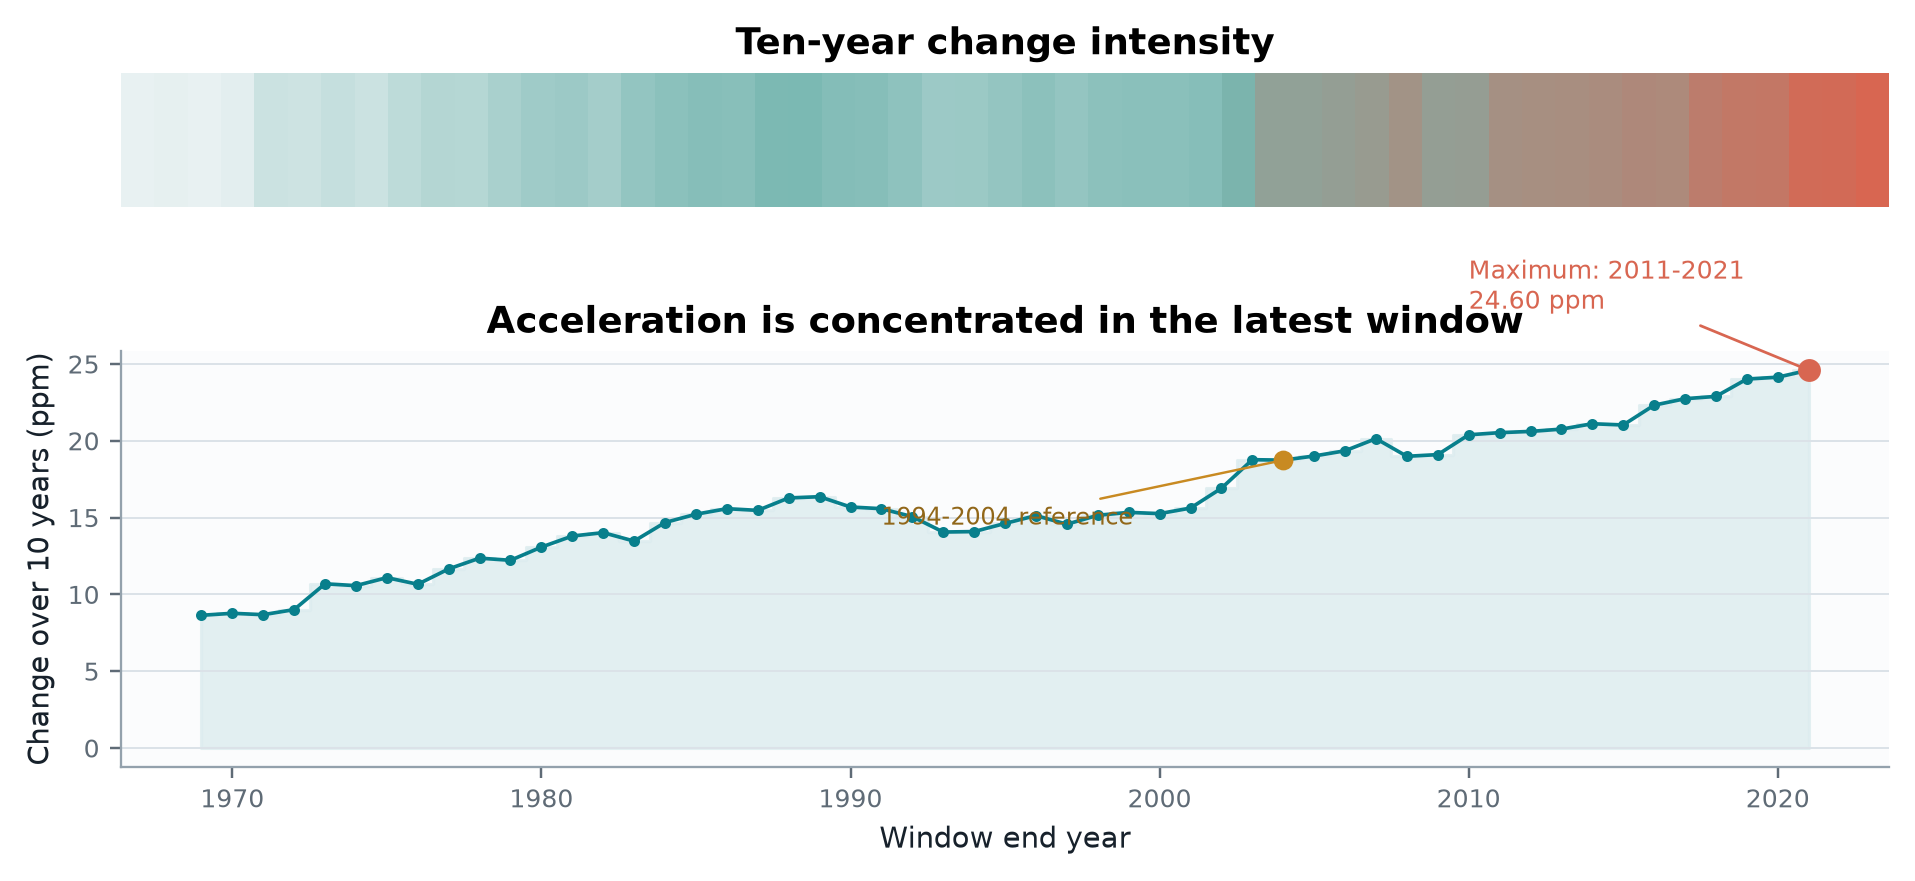
\includegraphics[width=0.88\textwidth]{../figures/fig2_tenyear.png}
\caption{All complete ten-year CO2 increases in the supplied annual series. The highlighted maximum is 2011--2021.}
\label{fig:rolling}
\end{figure}

The appendix lists all 53 windows. Publishing the full calculation matters here: it prevents a conclusion from depending on an unreported choice of endpoints.

\section{CO2 Trend Models}
\subsection{Linear Baseline}
The linear baseline is $\hat{C}_t=\beta_0+\beta_1t$. It is intentionally simple: its value is as a stable comparator, not as a claim that concentration growth must remain linear indefinitely. The fitted slope is 1.4766 ppm per year.

\subsection{Exponential Growth Comparator}
We fit $\hat{C}_t=a\exp(kt)$ where $t=0$ corresponds to 1959. The fitted values are $a=311.411$ and $k=0.004224$. This form captures smooth acceleration but becomes particularly sensitive in long extrapolations, so its 2100 value is reported as a scenario, not a precise forecast.

\subsection{Logistic Curve}
The logistic alternative is $\hat{C}_t=K/[1+\exp(-r(t-t_0))]$. It can represent eventual slowing, but the estimated midpoint (2422.9) is far beyond the observed range. That extrapolation warning is substantive: a flexible curve may fit the observations without identifying an interpretable future saturation point.

\subsection{ARIMA Increment Model}
For the differenced series, ARIMA(1,1,0) uses a drift and one autoregressive term: $\Delta C_t=d+\phi\Delta C_{t-1}+\varepsilon_t$. The fitted fallback calculation uses $d=0.8399$ and $\phi=0.4331$. It is a local time-series model, so it often validates better over a short future holdout while still being uncertain over many decades.

\begin{figure}[H]
\centering
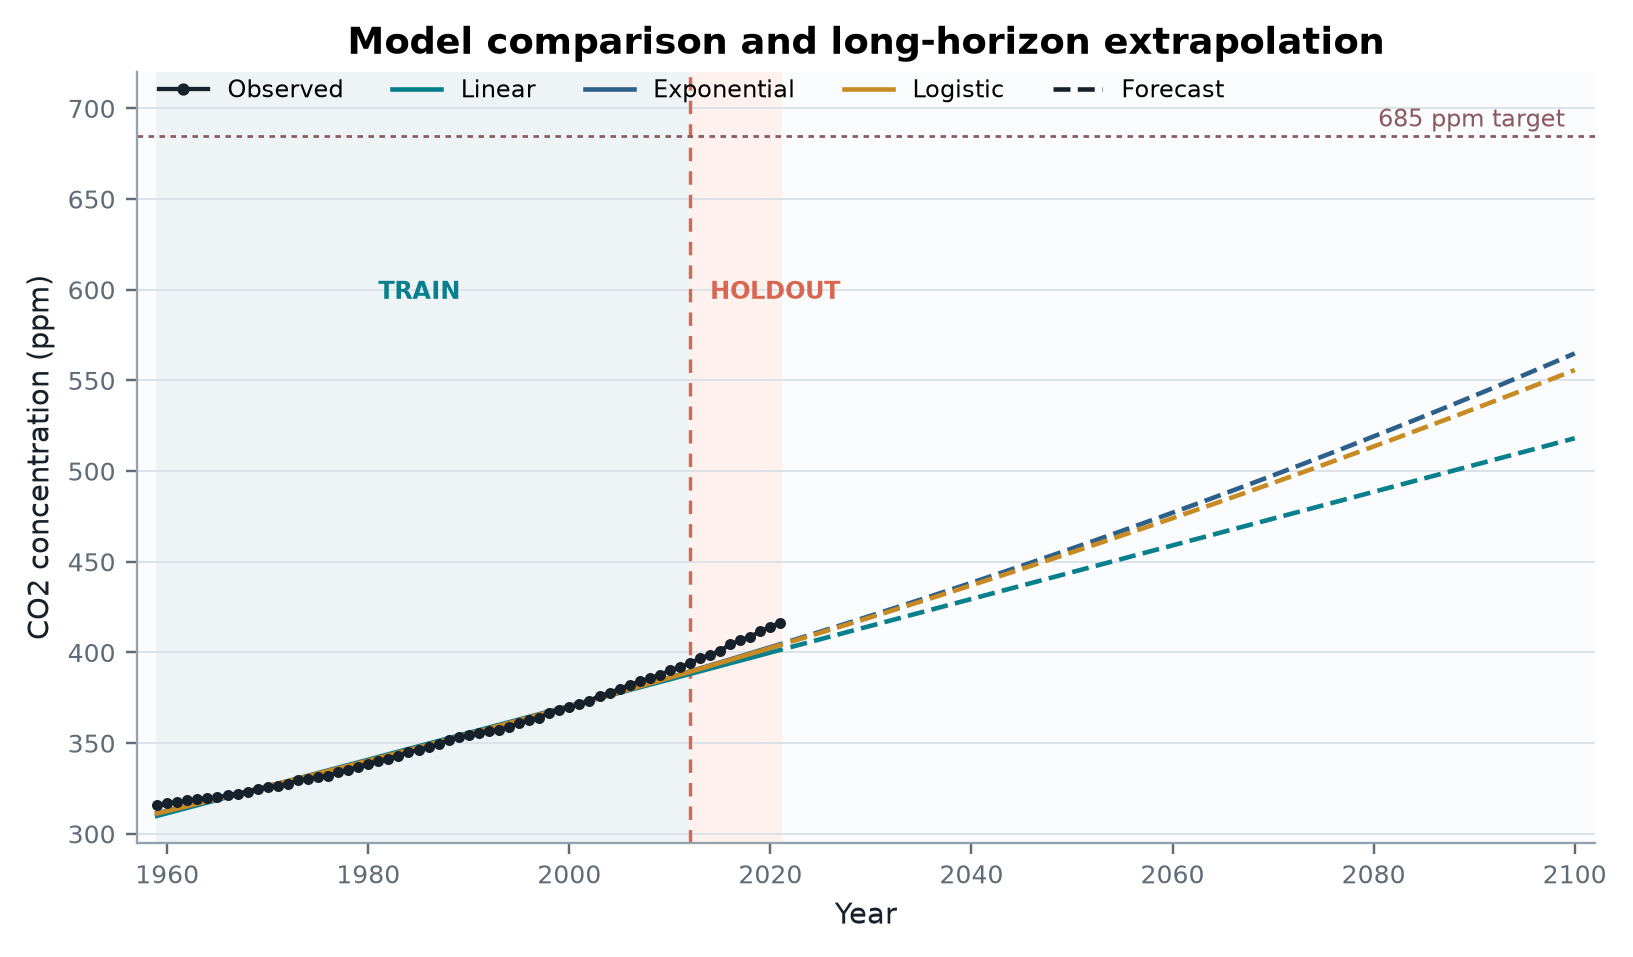
\includegraphics[width=0.88\textwidth]{../figures/fig1_co2_fits.png}
\caption{Four fitted CO2 continuations. Forecast differences widen with horizon because their structural assumptions differ.}
\label{fig:fits}
\end{figure}


\section{Validation and Forecast Comparison}
\subsection{Fixed Holdout Protocol}
We fit each CO2 model using 1959--2011 and reserve 2012--2021 for validation. For each held-out year, $e_t=C_t-\hat{C}_t$; RMSE is $\sqrt{n^{-1}\sum e_t^2}$ and MAE is $n^{-1}\sum |e_t|$. This is a stricter comparison than ranking only by in-sample residuals, because every model must forecast observations it did not use to calibrate itself.

\begin{table}[H]
\centering
\small
\begin{tabularx}{\textwidth}{lrrrr}
\toprule
Model & Holdout RMSE & Holdout MAE & 2050 ppm & 2100 ppm \\ \midrule
\midrule
Linear & 10.894 & 10.480 & 444.27 & 518.11 \\
Exponential & 8.584 & 8.242 & 457.36 & 564.90 \\
Logistic & 8.912 & 8.559 & 455.24 & 555.74 \\
ARIMA(1,1,0) & 5.884 & 5.097 & 459.98 & 534.06 \\
\bottomrule
\end{tabularx}
\end{table}


\subsection{Interpretation of the Comparison}
ARIMA(1,1,0) has the lowest ten-year holdout RMSE at 5.884 ppm. The exponential model is second at 8.584 ppm. This does not make ARIMA the uniquely correct model for 2100: the validation horizon is only ten years. Rather, the model spread is evidence of structural uncertainty. For 2050, the fitted range is 444.27--459.98 ppm; for 2100, it is 518.11--564.90 ppm. None of the four fitted forms reaches 685 ppm by 2050. This is a statement about these models and this data record, not a universal climate guarantee.

\subsection{Why the Holdout Is the Primary Comparison}
The fitting period ends in 2011, while the validation period begins in 2012. This boundary simulates the information available to a forecaster at the first prediction. The 2012--2021 observations are never used to estimate the coefficients reported in Table 3. The comparison therefore asks a concrete question: if the model had been stopped in 2011, how well would its continuation have reproduced the next decade?

The holdout is not intended to represent every possible future regime. Ten observations are still a small sample, and the period includes year-to-year fluctuations that are not explained by a smooth deterministic trend. We consequently use RMSE to rank short-run predictive performance, but use the cross-model envelope rather than one selected curve to communicate the 2050 and 2100 results. This prevents a good local forecast from being mistaken for evidence that the same model is structurally correct for an eighty-year extrapolation.

\subsection{Error Decomposition}
For each held-out year, the error is decomposed as
\begin{equation}
 e_t=C_t-\widehat C_t,\qquad
 \mathrm{RMSE}=\sqrt{\frac{1}{10}\sum_{t=2012}^{2021}e_t^2},\qquad
 \mathrm{MAE}=\frac{1}{10}\sum_{t=2012}^{2021}|e_t|.
\end{equation}
RMSE weights a large miss more heavily than MAE. This is useful because a model that systematically misses the upper end of the holdout may appear acceptable under average absolute error while still producing a materially different long-run continuation. Reporting both measures makes that choice visible.

\begin{table}[H]
\centering
\small
\caption{Interpretation of the four candidate structures.}
\begin{tabularx}{\textwidth}{lXX}
\toprule
Structure & What it preserves & Main extrapolation risk \\
\midrule
Linear & A constant annual increment & It cannot represent persistent acceleration or saturation. \\
Exponential & A constant proportional growth rate & Small rate errors compound rapidly by 2100. \\
Logistic & Growth followed by a finite asymptote & The asymptote and midpoint are weakly identified outside the sample. \\
ARIMA(1,1,0) & Local dependence in annual increments & Long-horizon behavior depends on a short differenced history. \\
\bottomrule
\end{tabularx}
\end{table}

\subsection{Forecast Bands as Structural Uncertainty}
The interval 518.11--564.90 ppm in 2100 is not a statistical confidence interval around a single data-generating process. It is a structural range generated by four deliberately different continuations. This range excludes parameter uncertainty, future changes in emissions, and physical climate feedbacks. Its value is diagnostic: the choice of functional form alone changes the answer by 46.79 ppm at the end of the horizon.

\section{Temperature Trend and Threshold Timing}
The fitted temperature line is $\hat{T}_t=\alpha_0+\alpha_1t$, with slope 0.01649 C per year. Its in-sample RMSE is 0.107 C and $R^2=0.891$. Inverting the fitted line gives the threshold times in Table 4. The intervals are calculated from the regression uncertainty and are reported because a decimal year alone would convey false precision.

\begin{table}[H]
\centering
\small
\begin{tabularx}{\textwidth}{lrrr}
\toprule
Threshold & Point year & 95 percent interval & SE (years) \\ \midrule
\midrule
1.25 C & 2044.2 & 2039.2--2049.3 & 2.57 \\
1.5 C & 2059.4 & 2053.1--2065.7 & 3.22 \\
2.0 C & 2089.7 & 2080.8--2098.6 & 4.53 \\
\bottomrule
\end{tabularx}
\end{table}


\begin{figure}[H]
\centering
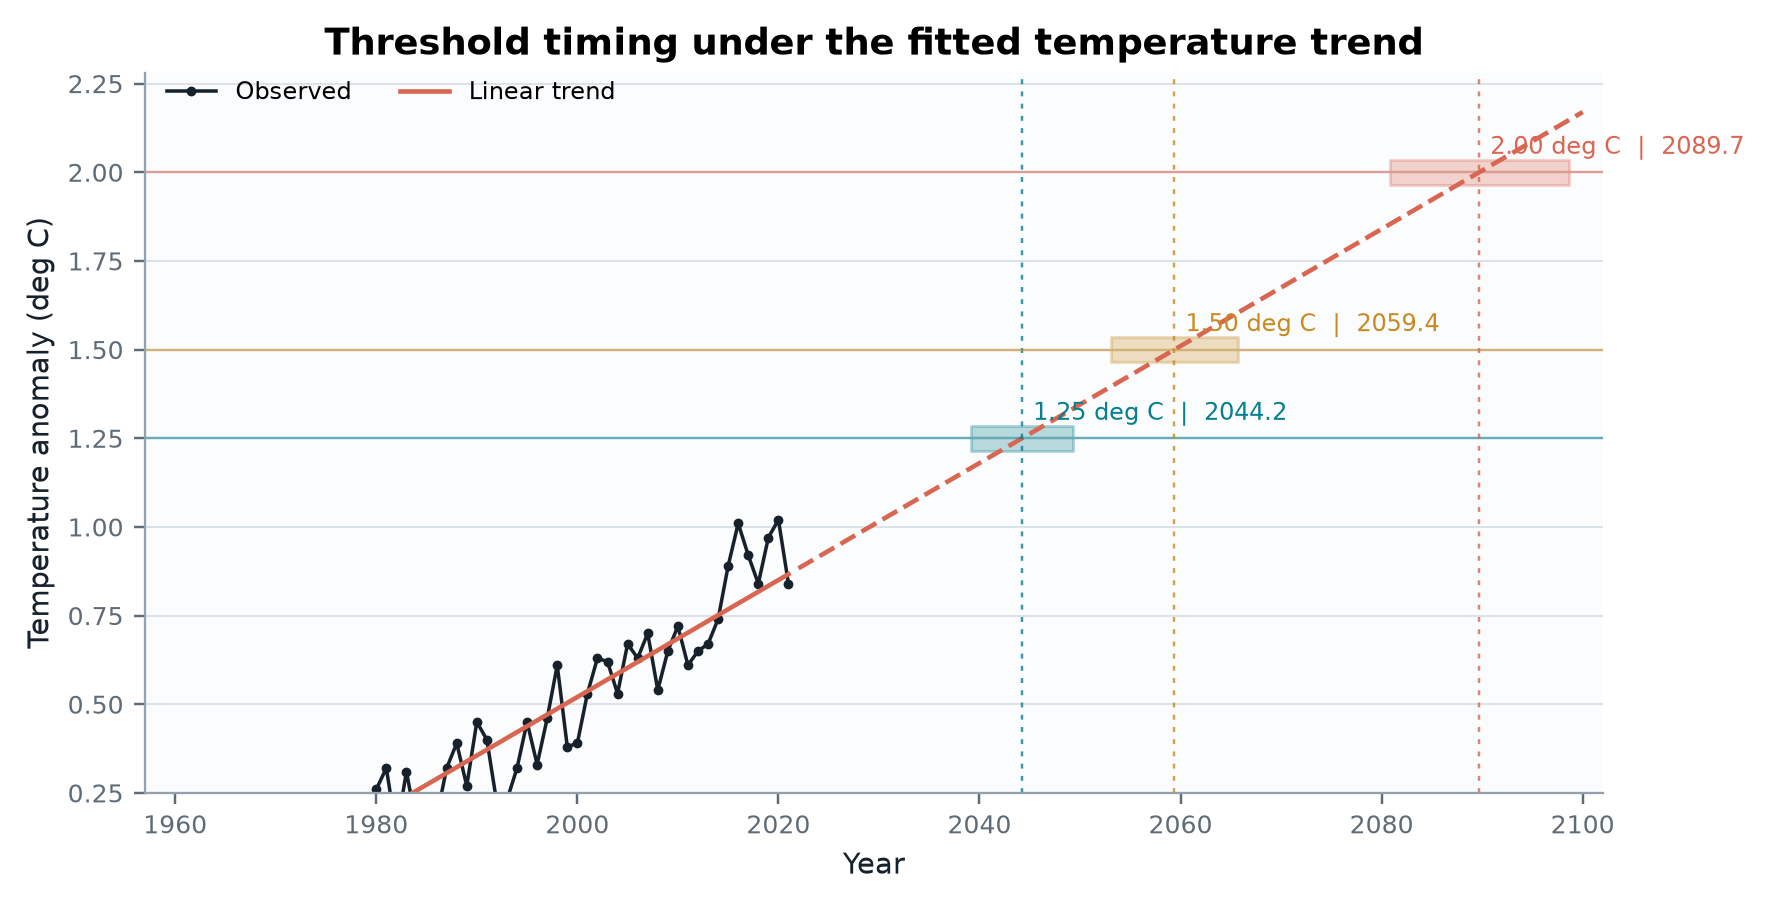
\includegraphics[width=0.88\textwidth]{../figures/fig4_temp_threshold.png}
\caption{Temperature-anomaly trend with the modeled threshold crossings and uncertainty windows.}
\label{fig:temperature}
\end{figure}

\subsection{Deriving the Threshold Years}
Let the fitted temperature trend be $\widehat T(y)=a+b(y-1958)$, where $y$ is the calendar year. For a threshold $q$, the crossing year is obtained by solving
\begin{equation}
 y_q=1958+\frac{q-a}{b}.
\end{equation}
The calculation uses the fitted line only; it does not mean that the observed climate system must cross the threshold monotonically. A warm year followed by a cool year can move an annual observation below a threshold even after the trend line has crossed it.

To quantify this limitation, we propagate uncertainty in the fitted coefficients through the inverse function. If the fitted coefficient vector is $\theta=(a,b)$ and $g(\theta)=1958+(q-a)/b$, then the first-order variance approximation is
\begin{equation}
 \mathrm{Var}(y_q)\approx \nabla g(\theta)\,\mathrm{Cov}(\theta)\,\nabla g(\theta),
 \qquad
 \nabla g=\left(-\frac{1}{b},-\frac{q-a}{b^2}\right).
\end{equation}
This explains why uncertainty grows for later thresholds: inversion divides by the trend slope, and the extrapolated point is farther from the observed sample.

\begin{table}[H]
\centering
\small
\caption{Practical reading of the temperature-threshold calculation.}
\begin{tabularx}{\textwidth}{lXX}
\toprule
Quantity & What the calculation says & What it does not say \\
\midrule
Point year & When the fitted annual trend equals the threshold & The exact year of every future annual observation \\
95 percent interval & Propagated uncertainty under the linear regression approximation & A complete climate-scenario uncertainty interval \\
Trend slope & Average change represented by the supplied record & A permanent physical warming rate \\
\bottomrule
\end{tabularx}
\end{table}


\section{Joint-Series Analysis: Association, Not Mechanism}
\subsection{Correlation}
On the 63 overlapping years, Pearson correlation is $r=0.9612$. Figure \ref{fig:scatter} visualizes this strong upward association. Both series also trend with calendar time, so the correlation is descriptive rather than a controlled estimate of a physical effect.

\begin{figure}[H]
\centering
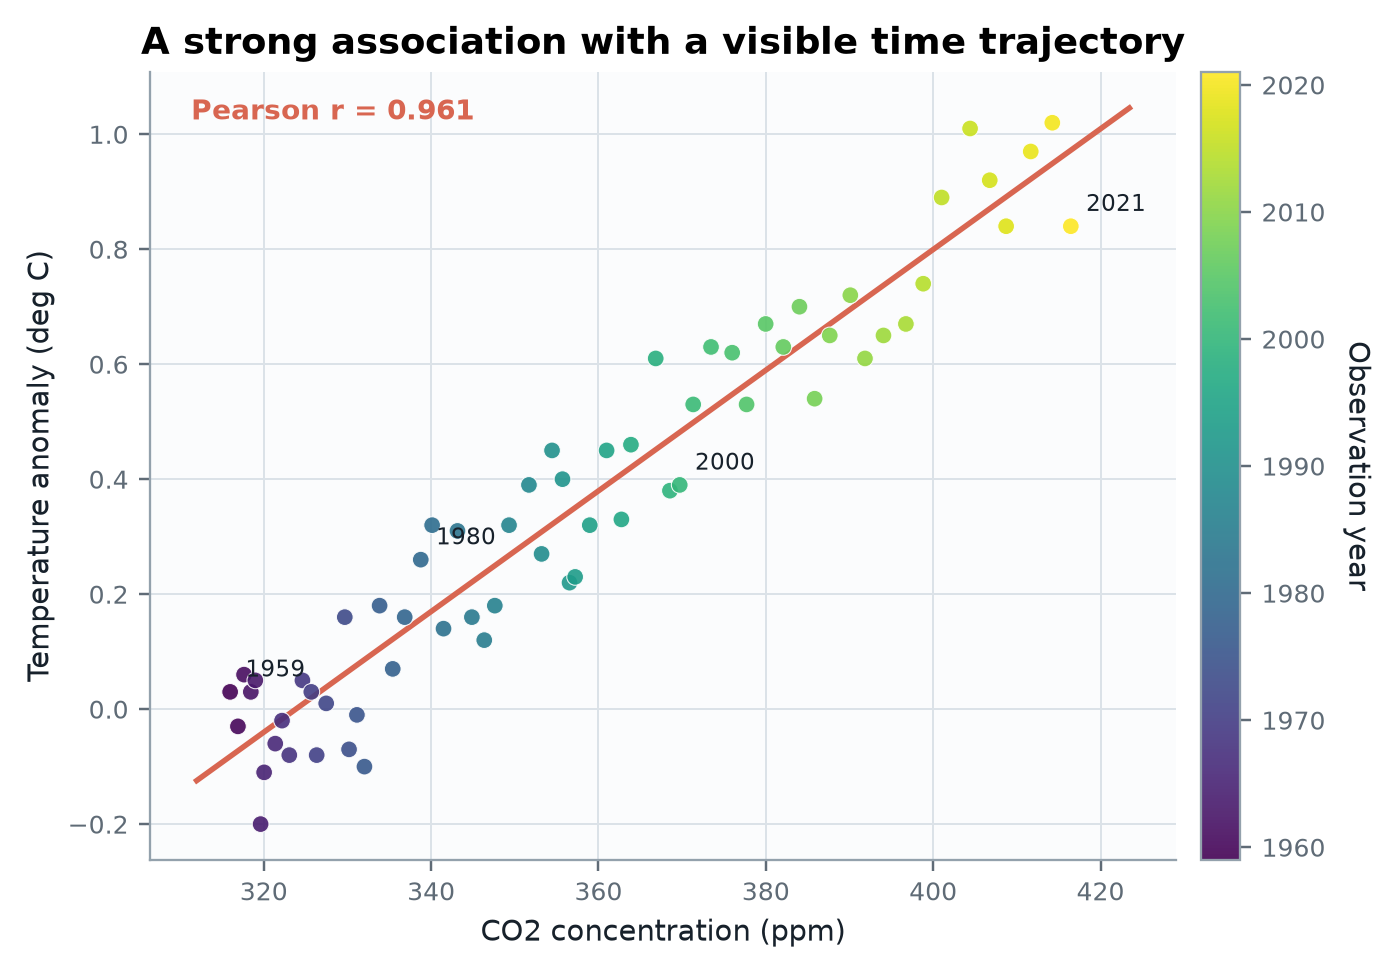
\includegraphics[width=0.74\textwidth]{../figures/fig3_scatter.png}
\caption{Aligned annual CO2 and temperature anomalies. The plot documents association but does not control for time or other forcings.}
\label{fig:scatter}
\end{figure}


\subsection{One-Lag Granger Statistic}
We compare a restricted temperature-increment regression with an unrestricted one that includes the previous CO2 increment. The CO2-to-temperature test has $F=39.514$ and $p=4.314e-08$; the reverse direction has $F=0.073$ and $p=0.789$. At this lag and in this data set, prior CO2 changes add predictive information for temperature changes while the reverse does not. This does not establish physical causation. The test is exploratory, includes only one lag, and omits key climate-system variables.

\subsection{Specification and Interpretation}
For clarity, the directional test compares two regressions for the temperature increment:
\begin{align}
 \Delta T_t&=c+\lambda\Delta T_{t-1}+u_t, &&\mathrm{restricted\ model},\\
 \Delta T_t&=c+\lambda\Delta T_{t-1}+\gamma\Delta C_{t-1}+v_t, &&\mathrm{unrestricted\ model}.
\end{align}
The null hypothesis is $\gamma=0$. The reverse test exchanges $C$ and $T$. Because both series contain strong time trends, the test is performed on increments rather than levels, reducing one obvious source of spurious significance. Nevertheless, differencing does not remove omitted variables, measurement issues, serial correlation concerns, or the possibility that both series respond to a common driver.

The appropriate conclusion is conditional and asymmetric: under this one-lag specification, lagged CO2 increments improve prediction of the next temperature increment, while lagged temperature increments do not improve the reverse prediction at the reported level. The word ``predict'' is essential. A predictive regression can be useful for forecasting without identifying a mechanism, and a non-significant reverse test cannot prove that no physical feedback exists.

\begin{table}[H]
\centering
\small
\caption{Guardrails for reading the joint-series results.}
\begin{tabularx}{\textwidth}{lX}
\toprule
Finding & Narrow interpretation \\
\midrule
$r=0.9612$ & The two aligned annual series move together over the sample. \\
$p=4.31\times10^{-8}$ in the forward test & Lagged CO2 increments add predictive content under one chosen specification. \\
$p=0.7886$ in the reverse test & The reverse lagged term is not useful under the same limited specification. \\
\bottomrule
\end{tabularx}
\end{table}

\section{Sensitivity and Reliability}
We perturb the exponential growth rate by minus 10 percent and plus 10 percent, holding its other fitted terms fixed. The resulting 2100 values are 532.24, 564.90, and 599.56 ppm. The spread is material even before considering alternative model structures.

\begin{figure}[H]
\centering
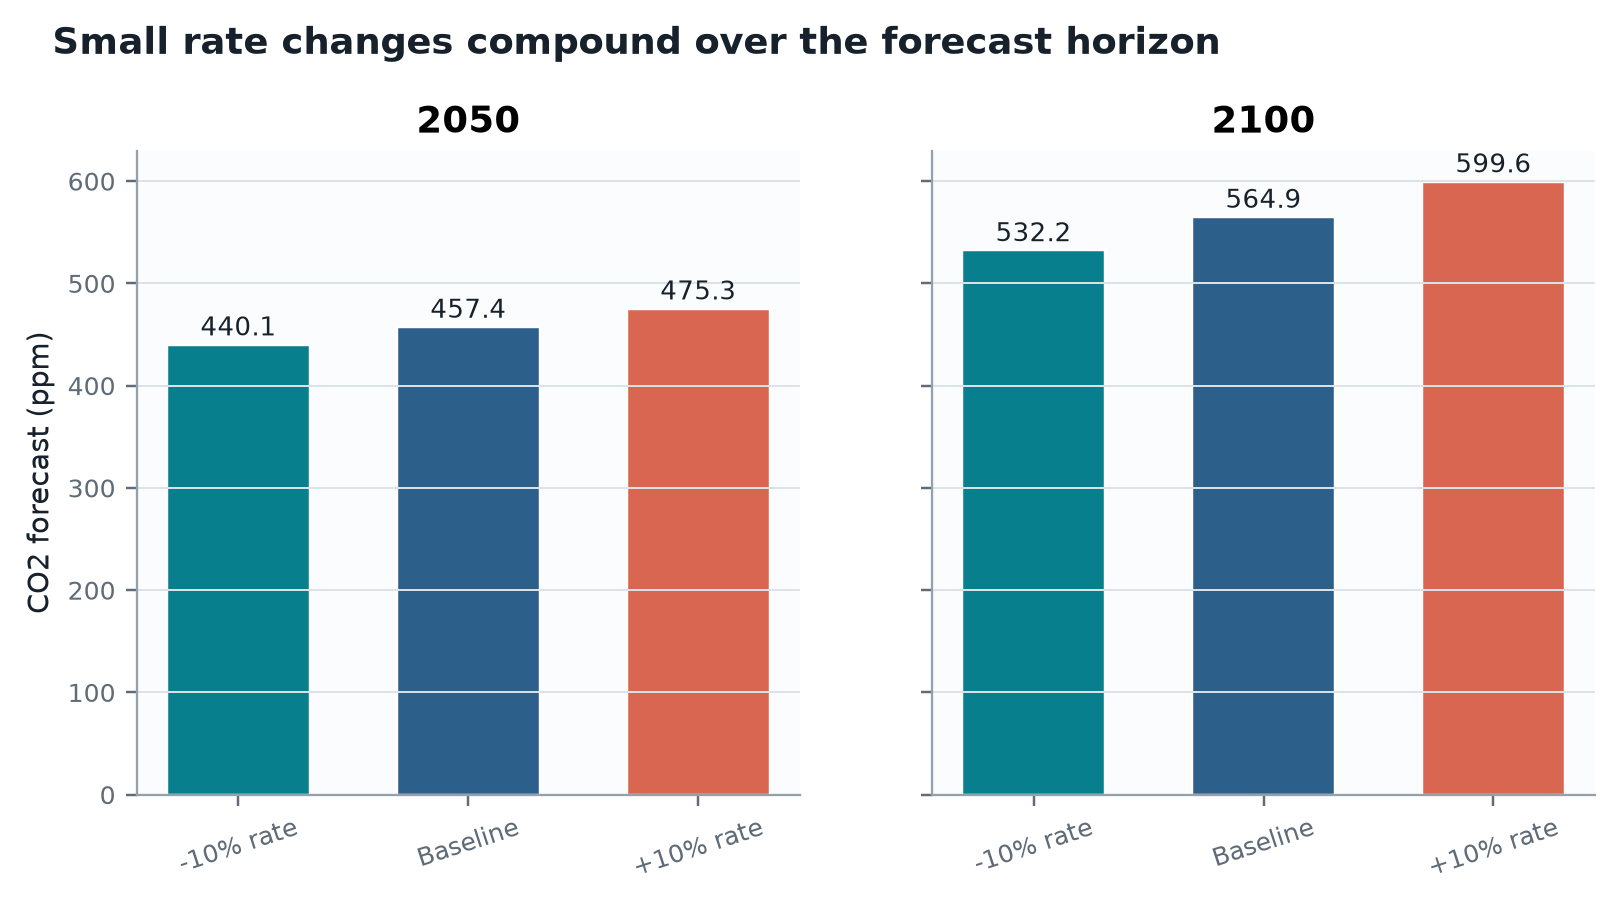
\includegraphics[width=0.88\textwidth]{../figures/fig5_sensitivity.png}
\caption{Exponential-model sensitivity when the fitted growth rate is perturbed by plus or minus 10 percent.}
\label{fig:sensitivity}
\end{figure}


\begin{table}[H]
\centering
\small
\begin{tabularx}{\textwidth}{lrr}
\toprule
Rate scenario & 2050 ppm & 2100 ppm \\ \midrule
\midrule
-10 percent & 440.11 & 532.24 \\
Baseline & 457.36 & 564.90 \\
+10 percent & 475.28 & 599.56 \\
\bottomrule
\end{tabularx}
\end{table}


\subsection{Strengths, Weaknesses, and Use Conditions}
The approach has three strengths: competing models make extrapolation uncertainty visible; a fixed holdout makes short-term accuracy testable; and all annual values and rolling calculations are published below. Its weaknesses are equally important. The records are short relative to the 2100 horizon; model selection can change with the validation window; the ARIMA and Granger routines are transparent local numerical fallbacks; and neither trend extrapolation nor Granger significance is a physical climate model. These results are therefore appropriate for comparative evidence and communication, not for policy-grade scenario design.

\subsection{Additional Sensitivity Questions}
Three sensitivity questions follow directly from the construction. First, changing the growth rate changes the exponential forecast multiplicatively, so the effect is small near 2050 but large by 2100. Second, changing the holdout boundary can change which model wins the short-run ranking; this is why we retain all four projections. Third, changing the threshold target affects both the numerator and the extrapolation distance in the inverse temperature calculation, so later thresholds should be read with wider caution.

\begin{table}[H]
\centering
\small
\caption{Sensitivity map for the reported conclusions.}
\begin{tabularx}{\textwidth}{lXX}
\toprule
Perturbation & Quantity most affected & Expected consequence \\
\midrule
Exponential rate $k$ & 2100 concentration & Compounding widens the scenario spread. \\
Holdout start year & RMSE and MAE ranking & The preferred short-run model may change. \\
Temperature threshold $q$ & Crossing year and uncertainty & Later thresholds require longer extrapolation. \\
Input endpoint & Ten-year maximum & The maximum window and comparison claim can change. \\
\bottomrule
\end{tabularx}
\end{table}

\subsection{Recommended Update Procedure}
When a new annual observation becomes available, the record should be appended without altering historical values. The ten-year-window audit should then be recomputed, followed by a fresh train--holdout split whose boundary is recorded. Each candidate model should be refit from the same snapshot, and the new forecast table should be compared with the previous one. Finally, the input fingerprint, metric fingerprint, and date of the update should be stored beside the paper. This procedure turns the document into an auditable rolling report rather than a one-time numerical claim.

\section{Conclusion}
The supplied CO2 record shows a pronounced acceleration in its rolling ten-year increases, culminating in a 24.60 ppm rise from 2011 to 2021. A single 2004-centered decade was not the maximum. On the common holdout, ARIMA(1,1,0) forecasts best among the four candidates, but the long-horizon conclusions are strongest when expressed as a range across structures: 518.11--564.90 ppm in 2100. The linked temperature analysis finds a strong association and an exploratory directional predictive signal, while carefully declining to label either as physical proof. The practical recommendation is to update the comparison as new annual data arrive and to replace pure trend extrapolation with emissions-pathway and physics-informed models whenever the decision stakes require it.

\section{Non-Technical Article: What the Numbers Actually Say}
\textbf{The CO2 curve is rising faster, but the future is not one number.} The annual record used in this study begins at 315.98 ppm of carbon dioxide in 1959 and reaches 416.45 ppm in 2021. When we compare every possible ten-year span, the biggest rise is not the interval ending in 2004. It is the 2011--2021 interval, which increases by 24.60 ppm.

We tested four common ways to extend the curve into the future. On the last ten observed years, a time-series model made the smallest average error. But the four models do not agree perfectly over a long horizon: their estimates for 2100 range from 518.11 to 564.90 ppm. None of these particular fitted models reaches 685 ppm by 2050. That is useful evidence, but it is not a promise about the planet. A curve fitted to old numbers cannot automatically account for future emissions choices, policy changes, volcanic eruptions, or feedbacks in the climate system.

The temperature record rises alongside CO2, and the two series are strongly associated. We also find that, in this limited annual data set, past CO2 changes help predict the next temperature change more than the reverse. That statistic is not proof that one measurement physically causes the other; climate science requires much richer evidence than a two-series regression. The honest takeaway is simple: the observed trend deserves attention, the uncertainty deserves equal attention, and future model updates should be checked against newly observed data.

\clearpage
\begin{thebibliography}{9}
\bibitem{data} Supplied HiMCM 2022 Problem B case data snapshot, \texttt{problem\_files/himcm\_data.csv}, accessed in the reproducible case workspace.
\bibitem{box} Box, G. E. P., Jenkins, G. M., Reinsel, G. C., and Ljung, G. M. \emph{Time Series Analysis: Forecasting and Control}. Wiley, 2015.
\bibitem{granger} Granger, C. W. J. ``Investigating Causal Relations by Econometric Models and Cross-spectral Methods.'' \emph{Econometrica}, 37(3), 1969, pp. 424--438.
\bibitem{ipcc} IPCC. \emph{Climate Change 2021: The Physical Science Basis}. Cambridge University Press, 2021.
\end{thebibliography}

\begin{appendices}
\section{Annual CO2 Observations}
The appendix preserves every supplied CO2 value used in the computations.
\begin{longtable}{rr}
\caption{Annual CO2 concentration used in this study.}\\
\toprule Year & CO2 (ppm) \\ \midrule
\endfirsthead
\toprule Year & CO2 (ppm) \\ \midrule
\endhead
1959 & 315.98 \\
1960 & 316.91 \\
1961 & 317.64 \\
1962 & 318.45 \\
1963 & 318.99 \\
1964 & 319.62 \\
1965 & 320.04 \\
1966 & 321.37 \\
1967 & 322.18 \\
1968 & 323.05 \\
1969 & 324.62 \\
1970 & 325.68 \\
1971 & 326.32 \\
1972 & 327.46 \\
1973 & 329.68 \\
1974 & 330.19 \\
1975 & 331.13 \\
1976 & 332.03 \\
1977 & 333.84 \\
1978 & 335.41 \\
1979 & 336.84 \\
1980 & 338.76 \\
1981 & 340.12 \\
1982 & 341.48 \\
1983 & 343.15 \\
1984 & 344.87 \\
1985 & 346.35 \\
1986 & 347.61 \\
1987 & 349.31 \\
1988 & 351.69 \\
1989 & 353.20 \\
1990 & 354.45 \\
1991 & 355.70 \\
1992 & 356.54 \\
1993 & 357.21 \\
1994 & 358.96 \\
1995 & 360.97 \\
1996 & 362.74 \\
1997 & 363.88 \\
1998 & 366.84 \\
1999 & 368.54 \\
2000 & 369.71 \\
2001 & 371.32 \\
2002 & 373.45 \\
2003 & 375.98 \\
2004 & 377.70 \\
2005 & 379.98 \\
2006 & 382.09 \\
2007 & 384.02 \\
2008 & 385.83 \\
2009 & 387.64 \\
2010 & 390.10 \\
2011 & 391.85 \\
2012 & 394.06 \\
2013 & 396.74 \\
2014 & 398.81 \\
2015 & 401.01 \\
2016 & 404.41 \\
2017 & 406.76 \\
2018 & 408.72 \\
2019 & 411.66 \\
2020 & 414.24 \\
2021 & 416.45 \\
\bottomrule
\end{longtable}

\section{Annual Temperature-Anomaly Observations}
The following table preserves every supplied annual temperature anomaly.
\begin{longtable}{rr}
\caption{Annual temperature anomaly used in this study.}\\
\toprule Year & Anomaly (C) \\ \midrule
\endfirsthead
\toprule Year & Anomaly (C) \\ \midrule
\endhead
1958 & 0.06 \\
1959 & 0.03 \\
1960 & -0.03 \\
1961 & 0.06 \\
1962 & 0.03 \\
1963 & 0.05 \\
1964 & -0.20 \\
1965 & -0.11 \\
1966 & -0.06 \\
1967 & -0.02 \\
1968 & -0.08 \\
1969 & 0.05 \\
1970 & 0.03 \\
1971 & -0.08 \\
1972 & 0.01 \\
1973 & 0.16 \\
1974 & -0.07 \\
1975 & -0.01 \\
1976 & -0.10 \\
1977 & 0.18 \\
1978 & 0.07 \\
1979 & 0.16 \\
1980 & 0.26 \\
1981 & 0.32 \\
1982 & 0.14 \\
1983 & 0.31 \\
1984 & 0.16 \\
1985 & 0.12 \\
1986 & 0.18 \\
1987 & 0.32 \\
1988 & 0.39 \\
1989 & 0.27 \\
1990 & 0.45 \\
1991 & 0.40 \\
1992 & 0.22 \\
1993 & 0.23 \\
1994 & 0.32 \\
1995 & 0.45 \\
1996 & 0.33 \\
1997 & 0.46 \\
1998 & 0.61 \\
1999 & 0.38 \\
2000 & 0.39 \\
2001 & 0.53 \\
2002 & 0.63 \\
2003 & 0.62 \\
2004 & 0.53 \\
2005 & 0.67 \\
2006 & 0.63 \\
2007 & 0.70 \\
2008 & 0.54 \\
2009 & 0.65 \\
2010 & 0.72 \\
2011 & 0.61 \\
2012 & 0.65 \\
2013 & 0.67 \\
2014 & 0.74 \\
2015 & 0.89 \\
2016 & 1.01 \\
2017 & 0.92 \\
2018 & 0.84 \\
2019 & 0.97 \\
2020 & 1.02 \\
2021 & 0.84 \\
\bottomrule
\end{longtable}

\section{All Complete Ten-Year CO2 Windows}
This audit table makes the rolling-window conclusion independently checkable.
\begin{longtable}{rrr}
\caption{Complete ten-year CO2 increases.}\\
\toprule Start year & End year & Increase (ppm) \\ \midrule
\endfirsthead
\toprule Start year & End year & Increase (ppm) \\ \midrule
\endhead
1959 & 1969 & 8.64 \\
1960 & 1970 & 8.77 \\
1961 & 1971 & 8.68 \\
1962 & 1972 & 9.01 \\
1963 & 1973 & 10.69 \\
1964 & 1974 & 10.57 \\
1965 & 1975 & 11.09 \\
1966 & 1976 & 10.66 \\
1967 & 1977 & 11.66 \\
1968 & 1978 & 12.36 \\
1969 & 1979 & 12.22 \\
1970 & 1980 & 13.08 \\
1971 & 1981 & 13.80 \\
1972 & 1982 & 14.02 \\
1973 & 1983 & 13.47 \\
1974 & 1984 & 14.68 \\
1975 & 1985 & 15.22 \\
1976 & 1986 & 15.58 \\
1977 & 1987 & 15.47 \\
1978 & 1988 & 16.28 \\
1979 & 1989 & 16.36 \\
1980 & 1990 & 15.69 \\
1981 & 1991 & 15.58 \\
1982 & 1992 & 15.06 \\
1983 & 1993 & 14.06 \\
1984 & 1994 & 14.09 \\
1985 & 1995 & 14.62 \\
1986 & 1996 & 15.13 \\
1987 & 1997 & 14.57 \\
1988 & 1998 & 15.15 \\
1989 & 1999 & 15.34 \\
1990 & 2000 & 15.26 \\
1991 & 2001 & 15.62 \\
1992 & 2002 & 16.91 \\
1993 & 2003 & 18.77 \\
1994 & 2004 & 18.74 \\
1995 & 2005 & 19.01 \\
1996 & 2006 & 19.35 \\
1997 & 2007 & 20.14 \\
1998 & 2008 & 18.99 \\
1999 & 2009 & 19.10 \\
2000 & 2010 & 20.39 \\
2001 & 2011 & 20.53 \\
2002 & 2012 & 20.61 \\
2003 & 2013 & 20.76 \\
2004 & 2014 & 21.11 \\
2005 & 2015 & 21.03 \\
2006 & 2016 & 22.32 \\
2007 & 2017 & 22.74 \\
2008 & 2018 & 22.89 \\
2009 & 2019 & 24.02 \\
2010 & 2020 & 24.14 \\
2011 & 2021 & 24.60 \\
\bottomrule
\end{longtable}

\section{Model Parameters and Diagnostic Record}

\begin{table}[H]
\centering
\small
\begin{tabularx}{\textwidth}{l l r X}
\toprule
Model & Parameter & Value & Interpretation \\ \midrule
\midrule
Linear & $\beta_1$ & 1.476640 & ppm per year \\
Exponential & $a$ & 311.411070 & 1959 amplitude \\
Exponential & $k$ & 0.00422366 & annual rate \\
Logistic & $K$ & 3134.8 & asymptote parameter \\
Logistic & $r$ & 0.00475402 & growth-rate parameter \\
Logistic & $t_0$ & 2422.86 & midpoint year \\
ARIMA & $d$ & 0.839927 & increment drift \\
ARIMA & $\phi$ & 0.433131 & lag-one coefficient \\
\bottomrule
\end{tabularx}
\end{table}

The source metric file records the SHA-256 fingerprint shown below; the input CSV has its own fingerprint. These values identify the exact result and data snapshots used to populate this document.
\begin{center}
\small metrics: 6bd37cf03a560021813977145bf702a40fa6350f4b34236b8455d589c6ff2fb5\\
input: 491b3bbe15e1162a19cc1e163f444030b27322b0586f7b10ab8443c52db1e58d
\end{center}

\section{Claim-to-Evidence Guide}

\begin{table}[H]
\centering
\small
\begin{tabularx}{\textwidth}{p{0.28\textwidth}p{0.22\textwidth}X}
\toprule
Claim & Evidence location & Qualification \\ \midrule
\midrule
Largest ten-year rise is 24.60 ppm & Figure 1 and Appendix C & Descriptive result from supplied record \\
ARIMA has lowest holdout RMSE & Table 3 & Fixed 2012--2021 holdout only \\
No fitted model reaches 685 ppm by 2050 & Table 3 & Not a universal climate guarantee \\
Temperature thresholds & Table 4 and Figure 4 & Linear trend with intervals \\
CO2-to-temperature predictive signal & Section 7 & Exploratory Granger statistic, not physical causation \\
\bottomrule
\end{tabularx}
\end{table}

\section{Reproducible Calculation Details}
This appendix records the calculation conventions used to transform the supplied annual observations into the reported statistics. Let $t=y-1959$ for the CO2 models. The linear coefficients are obtained by ordinary least squares, minimizing
\begin{equation}
 \mathrm{SSE}(\beta_0,\beta_1)=\sum_{y=1959}^{2021}
 \left[C_y-(\beta_0+\beta_1t_y)\right]^2.
\end{equation}
For the exponential comparator, taking logarithms gives $\log C_y=\log a+kt_y$; the fitted values are then returned to the original ppm scale before all errors are calculated. The logistic curve is fit in its original scale because logarithmic transformation does not linearize its three parameters in a way that remains numerically stable across the sample.

For the ARIMA increment model, the first difference is $D_t=C_t-C_{t-1}$. The fitted recurrence is $\widehat D_t=d+\phi D_{t-1}$, and the level forecast is reconstructed by $\widehat C_t=C_{t-1}+\widehat D_t$. This reconstruction is why the model is described as ARIMA$(1,1,0)$ rather than as a regression on the levels. Every reported forecast is rounded only for display; the error metrics use the unrounded calculation values.

\subsection{Holdout-Year Audit}
The following table records the observed CO2 values in the holdout and the corresponding forecast errors. It is included to show why the RMSE ranking is not based on a single unusually large observation.
\begin{longtable}{r r r r r r}
\caption{Holdout observations and model errors in ppm.}\label{tab:holdout-audit}\\
\toprule Year & Observed & Linear $e_t$ & Exp. $e_t$ & Logistic $e_t$ & ARIMA $e_t$ \\
\midrule
\endfirsthead
\toprule Year & Observed & Linear $e_t$ & Exp. $e_t$ & Logistic $e_t$ & ARIMA $e_t$ \\
\midrule
\endhead
2012 & 394.06 & 14.58 & 11.29 & 11.16 & 4.02 \\
2013 & 396.74 & 15.78 & 12.28 & 12.18 & 3.91 \\
2014 & 398.81 & 16.38 & 12.97 & 12.90 & 3.35 \\
2015 & 401.01 & 17.10 & 13.53 & 13.50 & 3.00 \\
2016 & 404.41 & 18.90 & 14.88 & 14.90 & 3.84 \\
2017 & 406.76 & 19.77 & 15.48 & 15.52 & 3.01 \\
2018 & 408.72 & 20.25 & 15.94 & 16.00 & 2.84 \\
2019 & 411.66 & 21.72 & 16.74 & 16.84 & 3.31 \\
2020 & 414.24 & 22.82 & 17.43 & 17.56 & 3.12 \\
2021 & 416.45 & 24.60 & 18.74 & 18.74 & 3.85 \\
\bottomrule
\end{longtable}
The error signs in this audit are defined as observed minus predicted. Positive values indicate that the fitted continuation was below the observation. The consistent positive sign for the smooth models is evidence that the late-period rise was stronger than their holdout continuation, while the local increment model follows that acceleration more closely.

\subsection{Increment Audit}
The annual increment $\Delta C_y=C_y-C_{y-1}$ is the local quantity used by the ARIMA model and the ten-year-window calculation. The selected rows below make the change in pace visible without replacing the full rolling-window table.
\begin{table}[H]
\centering
\small
\caption{Selected annual CO2 increments.}
\begin{tabularx}{\textwidth}{*{9}{>{\centering\arraybackslash}X}}
\toprule
Year & 1960 & 1970 & 1980 & 1990 & 2000 & 2010 & 2020 & 2021 \\
\midrule
$\Delta C_y$ (ppm) & 0.93 & 1.06 & 1.92 & 1.25 & 1.17 & 2.46 & 2.58 & 2.21 \\
\bottomrule
\end{tabularx}
\end{table}
The annual increments fluctuate substantially, so a ten-year comparison is more stable than a single-year comparison. At the same time, the endpoint increment in 2021 should not be interpreted as a new permanent rate. It is one observation inside the broader evidence chain.

\section{Decision Interpretation and Scenario Use}
The model outputs can support three different decisions, and each requires a different reading of uncertainty. For descriptive reporting, the measured 1959--2021 record and the rolling-window maximum are the strongest results because they do not require extrapolation. For near-term forecasting, the fixed holdout supports using ARIMA as the leading candidate, subject to updating the comparison when new observations arrive. For long-horizon planning, the structural range across models is more defensible than selecting the lowest-error model by habit.

\subsection{A Three-Layer Evidence Hierarchy}
\begin{enumerate}
\item \textbf{Observed layer.} Values in the supplied CSV, including the 24.60 ppm increase from 2011 to 2021, are direct record-based statements.
\item \textbf{Estimated layer.} Regression coefficients, holdout errors, correlation, and threshold years are calculations conditional on a specified sample and method.
\item \textbf{Scenario layer.} The 2050 and 2100 values are conditional continuations. They are useful for comparing model behavior, but they are not emissions scenarios or physical climate projections.
\end{enumerate}

Confusing these layers creates the most important communication risk in this study. In particular, the statement that no fitted curve reaches 685 ppm by 2050 belongs to the scenario layer. It must not be rewritten as a claim that atmospheric CO2 cannot reach that level under other emissions pathways or models.

\subsection{Updating the Scenario Envelope}
Suppose a new observation $C_{2022}$ is added. The first step is to calculate the new ten-year windows that end in 2022 and preserve the previous 2011--2021 result for historical comparison. The second step is to refit every candidate on a common training period and reserve a future holdout. The third step is to compare both the point forecasts and the width of the model envelope. A narrowing envelope can reflect genuine agreement, but it can also result from a shorter extrapolation horizon; it should not automatically be treated as increased certainty.

\begin{table}[H]
\centering
\small
\caption{Operational update checklist for a future data release.}
\begin{tabularx}{\textwidth}{lX}
\toprule
Step & Required record \\
1 & Input date, source path, row count, and file fingerprint. \\
2 & Complete ten-year windows and the identified maximum. \\
3 & Training years, holdout years, model parameters, RMSE, and MAE. \\
4 & 2050 and 2100 scenario values with model labels. \\
5 & Any changes to assumptions, limitations, or interpretation. \\
\bottomrule
\end{tabularx}
\end{table}

\subsection{Use Conditions}
The results are appropriate for a classroom modeling report, transparent comparison of statistical forms, and communication of why uncertainty matters. They are not sufficient by themselves for infrastructure design, emissions policy, or attribution of observed warming. Those applications would require additional predictors, physical constraints, uncertainty distributions, and external validation. This boundary is part of the model result, not an afterthought.

\section{Implementation Protocol}
The following protocol is a compact implementation specification for reproducing the analysis without relying on hidden spreadsheet operations. It is written as a sequence of deterministic operations so that a future update can be audited line by line.

\begin{enumerate}
\item Read the rows tagged CO2 and TEMP, convert year and value to numeric fields, and sort each series by year.
\item Check that each series has unique years and that the CO2 record covers 1959--2021. Do not interpolate missing observations silently.
\item For every CO2 start year $s$ for which $s+10$ is present, calculate $C_{s+10}-C_s$ and retain the start year, end year, and difference.
\item Set the training boundary to 2011. Fit all four candidate structures using exactly the training observations.
\item Generate one-step-ahead values for 2012--2021 using the same forecast convention for every candidate, then calculate RMSE and MAE.
\item Refit the selected descriptive forms on the complete historical record only when producing the stated 2050 and 2100 scenario continuations; record that refit choice explicitly.
\item Fit the temperature line on the supplied temperature record and invert it for each requested threshold.
\item Join CO2 and temperature by year over 1959--2021, then calculate correlation and the two one-lag increment tests.
\item Write the numerical output, input fingerprint, and assumptions to the result record before typesetting the paper.
\end{enumerate}

This order prevents information leakage. For example, calculating a model ranking after looking at the 2100 curves would make the holdout no longer a genuine validation. Separating model selection from long-horizon scenario display also makes it possible to explain why the lowest holdout error and the widest future range can coexist.

\subsection{Pseudocode}
The pseudocode below expresses the central calculation in a language-independent form.
\begin{table}[H]
\centering
\small
\caption{Reproduction pseudocode for the evidence chain.}
\begin{tabularx}{\textwidth}{p{0.18\textwidth}X}
\toprule
Stage & Operation \\
\midrule
Input & Load rows; filter by type; sort by year; preserve the original snapshot. \\
Windows & For $s$ in valid start years, append $(s,s+10,C_{s+10}-C_s)$; select the largest difference. \\
Split & Define training years as 1959--2011 and holdout years as 2012--2021. \\
Fit & Estimate linear, exponential, logistic, and ARIMA$(1,1,0)$ parameters on training data. \\
Score & For each model, compute held-out errors, RMSE, and MAE. \\
Project & Refit the stated continuation and evaluate each target year; retain model labels. \\
Joint test & Align years, difference both series, calculate correlation and one-lag directional tests. \\
Audit & Save inputs, parameters, metrics, figures, and limitations with fingerprints. \\
\bottomrule
\end{tabularx}
\end{table}

\subsection{Quality-Control Questions}
Before release, a reader should be able to answer yes to the following questions: Does every central number have a source observation or formula? Is the holdout separated before model comparison? Are all projected values labeled as scenarios? Does the appendix contain enough observations to detect a transcription error? Are predictive tests explicitly distinguished from causal claims? This checklist is deliberately stricter than visual polish because a clean-looking page cannot compensate for an untraceable number.

\subsection{Model Choice Under Different Objectives}
There is no single model that dominates for every objective. If the objective is to reproduce the next decade in this data snapshot, ARIMA$(1,1,0)$ is preferred because it has the smallest holdout RMSE. If the objective is to communicate a smooth proportional-growth scenario, the exponential form is easier to interpret through its rate parameter $k$. If the objective is to explore the possibility of eventual slowing, the logistic form provides a language for an asymptote, but its estimated midpoint lies far beyond the observed years and should not be treated as identified. The linear model remains valuable as a transparent lower-growth baseline.

This objective-dependent reading is preferable to declaring one curve ``the answer.'' Model selection is a decision rule tied to a loss function and a horizon. A short-horizon RMSE ranking answers a forecasting question; it does not answer a question about physical plausibility or policy scenarios. Keeping these purposes separate is why the paper reports both the ARIMA ranking and the full structural range.

\begin{table}[H]
\centering
\small
\caption{Recommended model reading by analytical objective.}
\begin{tabularx}{\textwidth}{lXX}
\toprule
Objective & Primary output & Appropriate caution \\
\midrule
Describe the supplied record & Observed values and ten-year audit & It is a historical statement, not a forecast. \\
Forecast a nearby decade & Holdout RMSE and MAE & The winning model may change as the holdout moves. \\
Compare long-run forms & 2050 and 2100 model envelope & The envelope is structural, not a confidence interval. \\
Discuss mechanisms & Joint-series diagnostics & Predictive evidence is not physical causation. \\
\bottomrule
\end{tabularx}
\end{table}

\section{Final Reading Guide}
The paper should be read from the measured record outward. Begin with the annual CO2 values and ten-year audit, which establish what happened in the supplied data. Next read the model comparison, where the fixed holdout identifies the best short-run continuation under the chosen protocol. Then read the projection range, where model disagreement becomes the principal uncertainty. Finally, read the temperature and joint-series sections, which add context while preserving the distinction between association, prediction, and mechanism.

The most defensible one-sentence summary is therefore: the supplied record shows increasing CO2 and a recent maximum ten-year rise, ARIMA performs best on the specified ten-year holdout, and long-term values remain conditional on model structure and future conditions. This summary is shorter than the paper, but it does not discard the qualifications that make the numerical claims honest.

\end{appendices}
\end{document}
